

%\section{Introduction}
%Modern nurse call systems should provide more than just sending a call to a nurse.


%\\ % We hereby propose a solution for this problem based on Notation3 rules.  %\\
%We use rule based reasoning on top of ontologies to implement this task.
%In a first attempt this problem was solved using an OWL \cite{OWL} ontology and SPARQL \cite{SPARQL} queries.
%To implement a nurse call system which meets these requirements, awareness of the context and  

%The solution we propose in this paper is based on an OWL \cite{OWL} ontology which we process using Notation3 \cite{notation3} rules.
%To implement a nurse call system which meets these requirements, we represented 




%\section{Background}\label{relwork}





\subsection{Business Case}\label{usecase}
Our business case is a nurse call system in a hospital.
The system is aware of certain details about personnel and patients.
Such information can include: personal skills of a staff member, staff competences, patient information, special patient needs, and/or the 
personal relationship between staff members and patients. %All this information is available in an OWL ontology. 
Furthermore, there is dynamic information available, as for example the current location of staff members and their status (busy or free). 
When a call is made, the nurse
call system should be able to assign the best staff member to answer that call. The definition of this ``best'' person
varies between hospitals and can be quite complex. 
Our system should thus be easily adjustable, but also very fast in taking a decision.
%\\
The system additionally controls different devices. If for example staff members enter a room with a patient, 
a decent light should be switched on; if they log into the room's terminal, they should have access to the medical lockers in the room. 
%
%By implementing such a system, 
Especially hospitals are interested in that kind of system as it enables them to organize their work 
%the work in a hospital can be organized 
in a more efficient way: 
\begin{itemize}
 \item Busy nurses get distracted less. They only receive a call if everyone else is also occupied or if the new task is more important than the task 
 they are currently performing.
 \item The system allows giving preference to staff members who are close to the caller. This prevents nurses from covering unnecessary big distances 
 in their anyhow stressful and physically exhausting 
 daily work.
 \item If the system is aware of the reason for a call, it can immediately assign nurses with the required skills. 
 Thus, no time is lost by first calling other staff members who then would have to ask for additional help.
 \item The system can prefer staff members who already know the patient and have a trust relationship with him. This increases the satisfaction of 
 the patient. At the same time, it also saves time for the caregiver, who is in such cases already familiar with the patient's needs and condition.
% \item The system keeps information about patients which can be assessed by the staff member called.
 \item The system is universal, i.e., electronic devices in the hospital can be controlled as well.
 \item The system is adaptable, i.e., hospitals can add their own requirements and priorities.
\end{itemize}

%Traditional nurse call systems don't take any patient-information into account. traditionally a patient makes a call and a random nurse responsible for the room gets the call.
%Our use case is different. We use all information available about a patient and the available nurses to always assign the best nurse (based on the current position of the nurse, the nurse's relation to the patient,
%competences, etc.) to the patient. Taking lots of information into account, such a system needs to be fast: especially in cases of emergencys the patient should not wait longer than number for the nurse.




\subsection{Technological Challenges}
\label{chal}
%Technological challenges - explaining why the business case is difficult to be solved by using traditional technologies

%Semantics: the system should be able to ``understand'' data and draw conclusions. \\
%Scalability: Huge datasets.\\
%Real-time: 5 seconds\\



An event-driven system as described above has to fulfill certain requirements. The system should:
%For the event driven system as described above we identified the following requirements:
%Below, we list the requirements (functional and non-functional) of the event-driven system of which we will devise a rule-based reasoning platform for. This system must
\begin{description}
%\item \emph{State} keep (consistent) state, which means it must be able to update data when an event is triggered,
\item[Scalability] cope with data sets ranging from 1000 to 100~000 relevant triple (i.e., triples necessary to be included for the reasoning to be correct);
\item[Semantics] be able to draw conclusions based on the information it is aware of;
\item[Functional complexity] implement deterministic decision trees with varying complexities; % from 1 to at least 6;
\item[Configuration] have the ability to change these decision trees at configuration time; and
\item[Real-time] return a response within 5 seconds to any given event.
\end{description}

%To meet these requirements different approaches can be taken.

%In a traditional hard coded system a fixed customized solution can be implemented. The main advantages of this approach are that they c 

There are several options to implement a nurse call system as described above. Following a more classical approach, the system could be written in 
an object-oriented programming language 
such as Java or C++. An implementation like this can easily fulfill the real-time and scalability constraints.
But such systems are traditionally hard-coded: they are implemented for a specific use case, and even though 
they might be able to support the required functional complexity, this implementation would be static. The possibility to configure complex decision trees
as postulated by the complexity requirement is rather hard to fulfill using traditional programming. Even more difficult to satisfy is the semantic requirement:
most object oriented languages do not support enough logic to ``understand'' the available information. Knowledge must be stated explicitly, 
as even simple connections between statements such as ``\textit{nurse x has location y}'' and ``\textit{y is location of nurse x}'' cannot be found easily.

Especially the last argument motivates us to solve the described problem using semantic web technologies as they natively fulfill the semantics requirement.
Knowledge can be represented in an OWL ontology which is understood by OWL-DL reasoners such as for example Pellet \cite{Pellet}. % or HermiT \cite{hermit}.
Complex decision trees can be handled by subsequent SPARQL queries. It is easy to add new queries or to change the order of existing queries 
and to thereby accommodate for the configuration constraint.
But our tests have shown that such systems inherently are not fast and reliable enough to fulfill the scalability and real-time requirements.
For bigger amounts of data or too complex decision trees, the reasoning times of traditional OWL-DL reasoners grow exponentially, which is not scalable.

To keep the benefits of an OWL-DL based implementation in a scalable and real-time way, we propose a rule-based solution.
By using OWL 2 RL rules and resolution instead of classical tableaux reasoning, we can significantly decrease reasoning times and still cover a major subset
of OWL 2. This approach benefits from the high performance of rule based reasoners. 
Even for bigger datasets the reasoning times are still faster than with the OWL-DL based approach. %very fast, as we will see later in this paper.  %and is able to reason very fast even over large datasets. 
%Because of its high performance (see benchmarks mentioned in \cite{eyepaper}), we chose the EYE reasoner for our purposes. As the reasoner is 
%able to cope with large datasets, our approach meets 
Also, complex decision trees can directly be implemented in rules. %, as those form the most natural 
As rules are the most natural representations of such trees, 
it is easy for a user to understand and change certain priorities 
or to configure new rules. A further advantage of our approach is that all logic is represented in one single way. Instead of
OWL plus SPARQL, we can implement the business case by only employing Notation3 Logic (N3). With the aforementioned system, we can meet all necessary requirements.
%, which makes our solution the 
%only one being able to fulfill all requirements.
%
%which form the most natu
%As this is the most natural representation
%Our implementation 
%Our solution is able to deal with 
%As the solution above, this implementation covers requirement \ref{sem}. 
%As we keep using 
%Our approach uses knowledge still makes use of 
%
%Our implementation makes use of OWL-RL rules written in Notation3. % \cite{notation3}.  
%As these rules enable us to cope with knowledge stored in OWL ontologies, our approach is general enough
%to be compatible with other semantic systems. 
%As the approach described above, requirement \ref{sem} 
%For our specific use case, OWL-RL was expressive 
%enough the provide the same results as a comparable OWL-DL based solution.
%
%Even though OWL-RL is less expressive than OWL-RL, this difference 
%had no influence to our use case. 
%Our system uses the EYE reasoner \cite{eyepaper} 
%The performance
%of the reasoner 
%whose high performance enables us to significantly increase the reasoning speed compared to an OWL-DL based solution.
%We additionally implemented the decision tree using rules. As rules are the natural representation of decision trees, 
%it is easy for the user to change certain priorities 
%or to add new rules.
%
%Instead of SPARQL-queries, a rule based solution can s


%PROS
%\begin{itemize}
% \item faster than owl
% \item one logic for all, no combination between OWL and query language
% \item EYE is very performant!
%\end{itemize}

 
 

%will especially have problems to meet the ``configuration''-requirement. A change in the decision tree would mean a change in the program code. 
%It is rather difficult to change 
%If a system is implemented in a traditional programming language for a specific use case it is 
%always difficult to change 


%Hard coded systems are not able to ``understand'' the data they are aware of. 


%A traditional hard coded system could not cope with

%A system as described above has to deal with a huge amount of knowledge, it has to reason about that knowledge and is must be able to update its own information 
%according to its conclusions (if a nurse is in a patients room, he is probably not ``free or available'' any more). As every hospital is different, 
%the rules or preferences in which kind of situation which nurse should be called also differs. 
%Our system should be easily adaptable. All this decisions must be taken real time.

%Traditional hard coded systems lack in particular the second last requirement: They are normally not flexible enough. A customized solution
%for a particular use case

%Traditional hard coded systems have problems to fulfill all the requirements mentioned above:
%Traditional hard coded systems are not flexible enough to fulfill these requirements. 
%The are not able to draw conclusions from huge datasets. 

%Although hard coded systems might be able to deal with a huge amount of data, they will not be 
%able to ``understand'' changes in the data and the possible consequences. Furthermore such systems lack the possibility to be changed at configuration time. Every new 
%requirement would require a new implementation of the system.

% Semantic based systems using purely OWL reasoning are on the other hand really good in 
% 
% 
% %Traditional hard coded systems can not easily incorporate all data needed. They are not flexible enough to ``understand'' complex situations. 
% %Rules which staff members should be called in what situations cannot be adapted that easily. 
% 
% Representing knowledge in OWL-ontologies is already an improvement but pure OWL-DL reasoning is too complex for this particular use case.
% Previous tests showed that by only using OWL-2 reasoners without any additional strategies we do not meet the time constraints
% of the real business use case. We need a powerful, but in the meantime fast solution.
% 
% 
% 
% 
% Analysis of the use case gave specifications as listed below.
% \begin{enumerate}
% \item Only a subset of the data is susceptible to change when an event is triggered, and this subset can be defined at initialization time. This subset is quite small (i.e., around $15\%$, irrespective of the total size of the data set), and is clearly defined as only a couple of classes and predicates that introduce dynamic data.
% \item There are events that trigger a state change before any reasoning needs to be done (e.g., a worker walks away from a certain location to another), and there are (similar) events that trigger a state change after the reasoning is done (e.g., a worker walks from his office to the complaint desk, meaning his status changes from 'free' to 'handlingClient').
% \item This reasoning system needs (thus) to be able to cope with state, and more specifically, be able to update a state based on reasoning.
% \item The change of a state is also part of a decision tree (e.g., when a worker is busy with a certain complaint, and he changes location, for example to get a file, consensus is needed whether his status changes from 'handlingClient' to 'away' or not. This consensus could be different for different companies).
% \end{enumerate}
% 
% Conclusions that can be drawn of these observations are as follows:
% \begin{enumerate}
% \item Preprocessing the static data at initialization time can give a significant performance gain, as this preprocessed optimized static data set can be reused every time an event is triggered.
% \item An event-driven reasoning system needs to be able to (programmatically) update the state of the data twice: once before the reasoning, and once after the reasoning. This preliminary update is necessary to avoid having conflicting data states (e.g., a worker being at two distinct locations at the same time when a reasoning occurs).
% \item This second update needs to keep track of the timestamp of when an event was triggered to cope with states that change through reasoning. explain better
% \item Each event actually introduces two reasoning runs: one for the actual reasoning over the event, and one to update the state. This second update also needs to be done by reasoning, as otherwise, the change between states is implemented programmatically, and can no longer be configured at configuration time.
% \end{enumerate}
% 
% Some specific other remarks due to the used technology stack:
% \begin{itemize}
% \item As the EYE-reasoner is a file-based process, the entire application needs to work file-based to persist its state. This also means that for every event, the current state needs to be updated in a file, which introduces some overhead compared to keeping the state in memory.
% \item As each event introduces two reasoning runs, this mean this file reading and writing overhead by EYE is doubled.
% \end{itemize}










\subsection{Rule-based Solution}\label{details}

%Technical details of the rule based solution

%Rule-based solution - technical details, esp. the usage of rules

%We use rules for two things: first to do owl-RL reasoning, second: to do the query. 
In this section, we further explain our solution in three parts.
First, we focus on the technical background and the technologies used. %give %an introduction into the technologies used and explain our choices. %first we give a brief introduction into N3 and the EYE-reasoner. 
In the second part we describe 
how we could improve reasoning times for our use case by employing OWL 2 RL rules written in N3. 
In the third part we show example rules from our decision trees and discuss options to change these rules. %, to give an idea how rules can be changed.

\subsubsection{Background}
Our solution improves on a more classical implementation which employs the OWL 2 reasoner Pellet \cite{Pellet}, and where
the decision tree was implemented via SPARQL queries.
All knowledge was represented using the ACCIO ontology\todo{name!}, which is described %a description is given 
by Ongenae et al. \cite{accioont}. 
Knowledge could either be fixed or dynamic, and updated via an event.
Fixed knowledge is, for example, information about skills of staff members, or patients' preferences.
Dynamic knowledge is, for example, the movement
of a nurse to a certain location, or a new call which is made by a patient.

%From the former implementation we keep the
Our new implementation keeps the knowledge representation of the first attempt but replaces SPARQL and OWL by Notation3 Logic (N3) \cite{N3Logic}.
%The only thing we keep from that former approach in our rule based implementation is 
%We have two kinds of knowledge, 
%We have two sources of knowledge: a static database translated into owl contains all information about staff, patients and physical devices which can be known beforehand. 
%Furthermore we
This logic forms a superset of \rdf and extends the \rdf data model by formulas (graphs), functional predicates, universal variables and logical operators, in particular
the implication operator. %extends the RDF model by adding formulas (literals which are graphs themselves), 
%variables, logical implication, and functional predicates. %, as well as providing an textual syntax alternative to RDF/XML.
These last two features enable the user to express rules. %can be understood by a reasoner.
As %a Notation3 
reasoner we use EYE \cite{eyepaper}, a semibackward reasoning engine enhanced with Euler path detection. 
The main reason for our choice is the high performance of the reasoner. Existing benchmarks and results are listed on the EYE website \cite{eye}. %Eye is especially
%
%The knowledge is represented in an OWL ontology \cite{accioont}
%Explain: Simple example. The reasoner needs a query.
%EYE \cite{eyepaper}.

%\subsection{Representing the knowledge}


\subsubsection{OWL 2 RL in N3}
%We started from an OWL-DL ontology which was used to 
%Possible data which can be processed by our system  
%The ACCIO Ontology
To be able to support OWL 2 RL reasoning in N3 we used the OWL 2 RL/\rdf rules as listed on the corresponding website~\cite{OWLRL}. 
Where possible, we made use of existing N3-translations of these rules as provided by EYE~\cite{EYEowl}. 
Missing concepts were added. Although the ACCIO ontology is designed for OWL-DL reasoning, the limitation to OWL RL had no impact for 
our specific use case. %, all derivations needed to cope with the desired decision trees were supported by OWL RL. 


\begin{lstlisting}[
  float=t,
  caption={OWL-RL rule for \texttt{rdfs:subClassOf} class axiom in N3.},
  label=lst:subclass]
§\textcolor{gray}{@prefix rdfs: <http://www.w3.org/2000/01/rdf-schema\#>.}§
§\textcolor{gray}{@prefix rdf: <http://www.w3.org/1999/02/22-rdf-syntax-ns\#>.}§

{?C rdfs:subClassOf ?D. ?X a ?C} => {?X a ?D}.
\end{lstlisting}
To illustrate the idea of using rules for OWL reasoning, we give a small example: Listing~\ref{lst:subclass} shows 
the class axiom rule\footnote{The rule is the N3 version of the cax-sco rule in Table 7 on the OWL 2 Profiles website~\cite{OWLRL}.} which is needed 
to deal with the rdfs concept
 \verb!subclassOf!. For convenience we omit the prefixes in the formulas below. The empty prefix refers to the ACCIO ontology, 
 \verb!rdf! and \verb!rdfs! have the same meaning as in Listing~\ref{lst:subclass}. Consider that we have the following T-Box triple stating that the class \verb!:Call!
 is 
 a subclass of the class \verb!:Task!:
 %If the ontology contains the triples
\[
 \verb!:Call rdfs:subClassOf :Task.! \tag{1}\label{1}
\]
If the A-Box contains an individual which is member of the class \verb!:Call!
\[\verb! :call1 a :Call.! \tag{2}\label{2}\]
%a rule based reasoner can use the rule given in listing \ref{lst:subclass} to conclude 
an OWL DL reasoner would make the conclusion that the individual also belongs to the class \verb!Task! 
\[
 \verb!:call1 a :Task.! \tag{3}\label{3}
\]
Our rule in Listing \ref{lst:subclass} does exactly the same: as Formula~\ref{1} and Formula~\ref{2} can be unified with the antecedence of the rule, a reasoner derives
the triple in Formula~\ref{3}. Other concepts can be handled similarly.







\subsubsection{Decision Trees }




 


%REMARK: Still not sure whether we need this section?
%The decision trees which have to be implement
%As mentioned above, decision trees as needed in for real life use cases can be quite complex. 

%Depending on the amount of available information, decision trees for nurse call systems can be quite complex. The ACCIO ontology 
%supports a huge variety of different concepts. %It is possible to model the profile of a patient (among others the 
 
The ACCIO ontology~\cite{accioont} provides the user with a huge variety of concepts which can, e.g., be used to describe patients (social background, needs, disease), 
staff members (skills, relationships to patients), and situations (locations of persons, states of devices). If all this information is actually available, decision trees
can use all of it and be therefore quite complex. In this section we provide two simple rules which could be part of such a tree and we explain how these rules can
be modified depending on the needs of an individual hospital.
 
 \begin{lstlisting}[
  float=t,
  caption={Rule assigning a preference value to a staff member with status "free" who is close to the call-location. },
  label=lst:ex]
§\textcolor{gray}{@prefix : <http://ontology/Accio.owl\#>.}§
§\textcolor{gray}{@prefix rdf: <http://www.w3.org/1999/02/22-rdf-syntax-ns\#>.}§

{
  ?c rdf:type :Call.
  ?c :hasStatus :Active. 
  ?c :madeAtLocation ?loc. 
  ?p :hasRole [rdf:type :StaffMember].
  ?p :hasStatus :Free.
  ?p :closeTo ?loc.
}
=>
{
  (?p ?c) :assigned 200.
}.
\end{lstlisting}
 
Listing~\ref{lst:ex} shows a rule which, given an active call, assigns a staff member with a certain preference to that call. The EYE reasoner works 
with filter rules (queries), it is easy to search for the assignment of a staff member with the lowest or highest number. 
In our example, lower numbers mean higher preferences. The antecedence of the given rule contains certain constraints: the active call is made on a certain location and
there is a staff member, who is currently free and close to that location. In such a case, our rule assigns the number 200 to the combination of call and staff member.

\begin{lstlisting}[
  float=t,
  caption={Rule assigning a preference value to a busy staff member who has the needed skills to answer the call. },
  label=lst:ex2]
§\textcolor{gray}{@prefix : <http://ontology/Accio.owl\#>.}§
§\textcolor{gray}{@prefix rdf: <http://www.w3.org/1999/02/22-rdf-syntax-ns\#>.}§

{
  ?c rdf:type :Call.
  ?c :hasStatus :Active.
  ?c :hasReason [rdf:type :CareReason].
  ?p rdf:type :Person.
  ?p :hasStatus :Busy.
  ?p :hasRole [rdf:type :StaffMember].
  ?p :hasCompetence [rdf:type :AnswerCareCallCompetence].
}
=>
{
  (?p ?c) :assigned 100.
}.
\end{lstlisting}








Listing~\ref{lst:ex2} displays another rule: here, the reason of the active call is known. We have a staff member who has the required 
skills to answer that kind of calls, but this staff member is currently busy. Our rule assigns the number 100 to this
combination of call and staff member. This means, in our current decision tree, we prefer this assignment to the one described by Listing~\ref{lst:ex}.

Now, it could be, that another hospital has different priorities. Imagine for example that in this new hospital, no busy staff should be called 
if there is still a free staff member available, regardless of the reason of the call. We could easily adapt our decision tree by simply changing the assignment number 
of one of the rules. If we replace the triple \[\verb! (?p ?c) :assigned 100.!\] in line 16 of Listing \ref{lst:ex2} by the triple \[\verb! (?p ?c) :assigned 300.!\]
the reasoner would prefer the assignment expressed by Listings \ref{lst:ex} to~\ref{lst:ex2}.

 
Similarly, we can add extra conditions to the rules. Currently, the rule in listing \ref{lst:ex2} does not take the location of the staff member into account. We can
change that by only adding the triples 
\[ \verb!?c :madeAtLocation ?loc. ?p :closeTo ?loc.!\]
to the antecedence of the rule. To give this new rule a higher priority than the existing one, we would again only have to change the assigned number in the consequence.
Rules with the same number are treated equally.















\subsection{Results}\label{ev}
%Results - the benefits of the solution, including improvement of KPIs


We compared the reasoning times of our implementation with the results of our former implementation using 
the Pellet reasoner and subsequent SPARQL-queries. 
As a joint test set up we ran a sequence of events, which we list below, the expected reasoning result is indicated in brackets. 

\begin{enumerate}
\item %[Launch Call] 
A patient launches a call (\emph{assign nurse and update call status})
\item
%[Redirected Call] 
The assigned nurse indicates that she is busy (\emph{assign other nurse})
\item
%[Temporarily Accept Call] 
The newly assigned nurse accepts the call task (\emph{update call status})
\item %[Corridor] 
The nurse moves to the corridor (\emph{update location})
\item %[Patient room] 
The nurse arrives at the patients' room (\emph{update location, turn on lights  and update nurse status})
\item %[Log in] 
The nurse logs into the room's terminal (\emph{update status call and nurse, open lockers})
\item %[Log off] 
The nurse logs out again (\emph{update status call and nurse, close lockers})
\item %[Corridor] 
The nurse leaves the room (\emph{update location and call status and turn off lights})
\end{enumerate}

We tested this set-up for two datasets, one dataset consisting of the nurses, hospital rooms and patients of one single ward, the other one for 10 wards.
Figure~\ref{fig:summary} shows the difference in reasoning times of this use case on the same hardware settings\footnote{Debian ``'Wheezy'', Intel(R) Xeon(R) CPU E5620@2.40GHz, 12GB RAM}, using two different technology stacks: the Pellet+SPARQL installation vs. the EYE installation\footnote{Pellet 3.0 and OWL-API 3.4.5 vs. EYE 7995 and SWI-Prolog 6.6.6}.
The timings shown are the sum of all reasoning cycles.

As the figure shows, the reasoning times of EYE are almost one order of magnitude better than the reasoning times of Pellet+SPARQL. 
When we review the reasoning times per call for one ward (Figure~\ref{fig:results1ward}), we see that the EYE installation has far 
more predictable reasoning times, as it is more robust against more complex decision trees
(e.g., the decision trees of the first two events are notably more complex than the other events' decision trees).
Pellet+SPARQL is much faster than EYE in the third event, because this event does not trigger any reasoning for Pellet+SPARQL, however, 
%in the EYE implementation a full reasoning cycle is performed for every incoming event.
a full reasoning cycle is performed by EYE. 
With an average reasoning time of about 2 seconds, the real-time constraint is achieved within small-scale datasets.

%\begin{figure}
% \small
% \begin{tabular}{p{1.3cm} p{1cm} p{1cm}}
% \hline
% \# wards & EYE & Pellet\\
% \hline
% \hline
% 1 & 18 & 79\\
% 10 & 288 & 2~124\\
% \hline
% \end{tabular}
% \normalsize
%\end{figure}



% \begin{figure}
% \begin{center}
% \includegraphics[width=0.7\textwidth]{Rplot18.jpeg}
% \end{center}
% \caption{Comparison of reasoning times of the individual events for 1 ward. EYE is generally faster, and more predictable.}
% \label{fig:results1ward}
% \end{figure}












%   \begin{figure}[!ht]\centering
% %  \CenterFloatBoxes
%  % \begin{floatrow}
%     \subfloat[Sum of reasoning times. % in seconds.
%     \label{fig:summary}]{
% % \begin{tabular}[b]{|l| r | r |}
% % \hline
% %  & 1 ward & 10 wards \\
% %  \hline
% %  \hline
% %  Pellet + SPARQL & 78.9 s & 2~124.1 s\\
% %  \hline
% %  EYE & 17.7 s & 287.7 s \\
% %  \hline
% %  \multicolumn{1}{c}{} \\
% %  \multicolumn{1}{c}{}
% % \end{tabular}
% 
% \small
% \begin{tabular}[b]{p{1.4cm} p{1cm} p{1cm}}
% \hline
% 
% No. of & \multicolumn{2}{c}{Time in sec.}\\
% %wards &\multicolumn{2}{c}{(in sec)} \\
%  wards & EYE & Pellet\\
% \hline
% \hline
% 1 & 18 & 79\\
% 10 & 288 & 2~124\\
% \hline
% &&\\
% &&\\
% &&\\
% \end{tabular} 
% \
% % \begin{tabular}[b]{|l| r | r |}
% % \hline
% %  & 1 ward & 10 wards \\
% %  \hline
% %  \hline
% %  Pellet + SPARQL & 78.9 s & 2~124.1 s\\
% %  \hline
% %  EYE & 17.7 s & 287.7 s \\
% %  \hline
% %  \multicolumn{1}{c}{} \\
% %  \multicolumn{1}{c}{}
% % \end{tabular}
% 
% \normalsize
% 
%     }\hfill
%     \subfloat[1 ward, reasoning time per event.\label{fig:results1ward}]{%
%       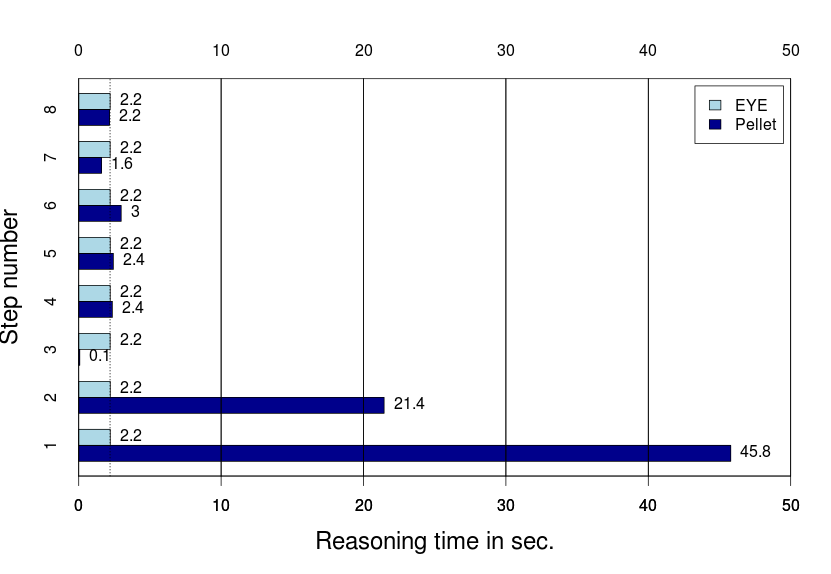
\includegraphics[width=0.6\textwidth]{Rplot14.png}
%     }
%     \caption{Comparison of reasoning times. EYE is generally faster, and more predictable.}
%     \label{figure:results} %\end{floatrow}
%   \end{figure}
  
 \begin{figure}
\centering
\begin{subfigure}{.4\textwidth}
  \centering
  {
% \begin{tabular}[b]{|l| r | r |}
% \hline
%  & 1 ward & 10 wards \\
%  \hline
%  \hline
%  Pellet + SPARQL & 78.9 s & 2~124.1 s\\
%  \hline
%  EYE & 17.7 s & 287.7 s \\
%  \hline
%  \multicolumn{1}{c}{} \\
%  \multicolumn{1}{c}{}
% \end{tabular}

\small
\begin{tabular}[b]{p{1.4cm} p{1cm} p{1cm}}
\hline

No. of & \multicolumn{2}{c}{Time in sec.}\\
%wards &\multicolumn{2}{c}{(in sec)} \\
 wards & EYE & Pellet\\
\hline
\hline
1 & 18 & 79\\
10 & 288 & 2~124\\
\hline
&&\\
&&\\
&&\\
\end{tabular} 
\
% \begin{tabular}[b]{|l| r | r |}
% \hline
%  & 1 ward & 10 wards \\
%  \hline
%  \hline
%  Pellet + SPARQL & 78.9 s & 2~124.1 s\\
%  \hline
%  EYE & 17.7 s & 287.7 s \\
%  \hline
%  \multicolumn{1}{c}{} \\
%  \multicolumn{1}{c}{}
% \end{tabular}

\normalsize

    }
  \caption{Sum of reasoning times.}
  \label{fig:summary}
\end{subfigure}%
\begin{subfigure}{.6\textwidth}
  \centering
  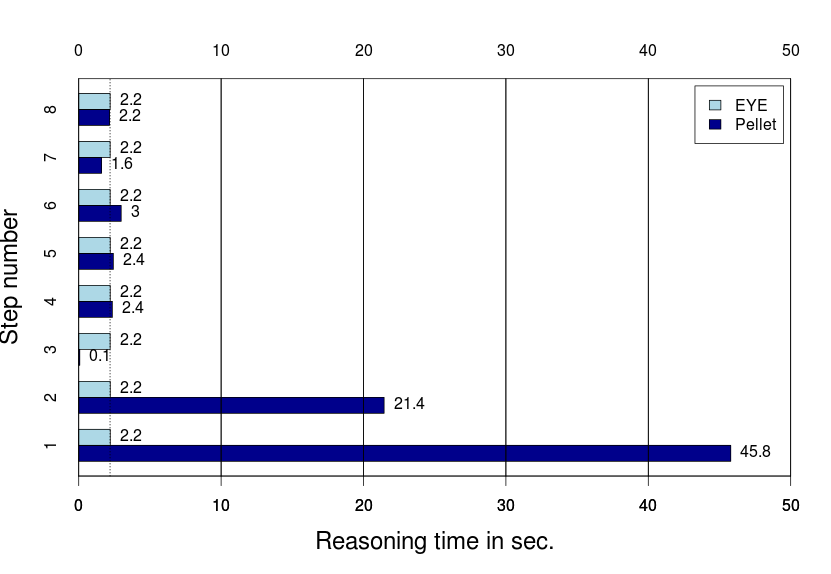
\includegraphics[width=\linewidth]{Rplot14.png}
  \caption{1 ward, reasoning time per event.}
  \label{fig:results1ward}
\end{subfigure}
\caption{Comparison of reasoning times. EYE is generally faster, and more predictable.}
\label{figure:result}
\end{figure} 
  
  
  
%     \begin{figure}[!ht]
%    \subfloat[1 ward\label{subfig-1:dummy}]{%
%       \begin{tabular}[t]{ccc}
% \hline
% \# wards & EYE & Pellet\\
% \hline
% \hline
% 1 & 18 & 79\\
% 10 & 288 & 2~124\\
% \hline
% \end{tabular}
%     }
%     \hfill
%     \subfloat[10 wards\label{subfig-2:dummy}]{%
%       \includegraphics[width=0.4\textwidth]{Rplot15.png}
%     }
%     \caption{Comparison of reasoning times of the individual events. EYE is generally faster, and more predictable.}
%     \label{table:results}
%    
%   \end{figure}
  
  
 
  

  
  
	


% 
% \begin{figure}
% \centering
% \begin{minipage}[t]{.4\textwidth}
% \centering
% \vspace{0pt}
% \includegraphics[width=0.5\textwidth]{Rplot15}
% \caption{This is the caption for figure}
% \end{minipage}\hfill
% \begin{minipage}[t]{.4\textwidth}
% \centering
% \vspace{0pt}
% \captionof{table}{This is the caption for table}
% \begin{tabular}{cc}
% 1 & Item 1 \\
% 3 & Item 2 \\
% 4 & Item 3 \\
% 5 & Item 4 \\
% 5 & Item 5 \\
% \end{tabular}
% \end{minipage}
% \end{figure}
%

  
  
  
  
  
%   \begin{figure}
%   \begin{minipage}[b]{0.6\linewidth}
%     \centering
%     %\includegraphics[width=\linewidth]{example-image}
% 
%  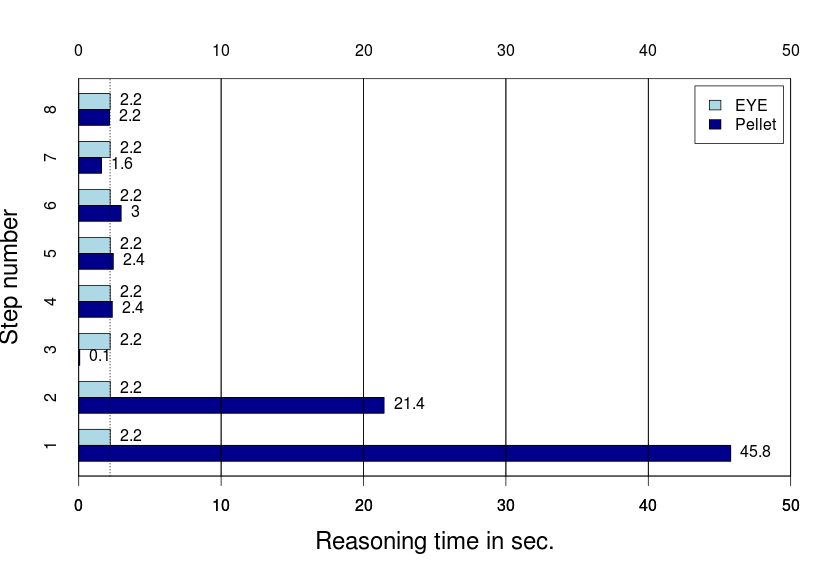
\includegraphics[width=\textwidth]{Rplot14}
% %\hspace{3cm}
%     %\rule{6cm}{6cm} %to simulate an actual figure
%   \caption{Comparison of reasoning times for individual events, 1 ward. EYE is generally faster, and more predictable.}  \label{fig:results1ward}
%   \end{minipage}%
%   \begin{minipage}[b]{0.3\linewidth}
%     \centering
%     \small
% \begin{tabular}{p{1cm} p{1cm} p{1cm}}
% \hline
% Wards & EYE & Pellet\\
% \hline
% \hline
% 1 & 18 & 79\\
% 10 & 288 & 2~124\\
% \hline
% &&\\
% &&\\
% \end{tabular} 
% \normalsize
% \caption{Comparison of the overall reasoning time for both, 1 and 10 wards. Values in seconds.}\label{fig:summary}
% \end{minipage}
% 
% \label{fig:test}
% \end{figure}
  
  
  
  
  
  
%   
  
%  \begin{figure}
%         \centering
%         \begin{subfigure}[b]{0.5\textwidth}
% \small
% \begin{tabular}{p{1.3cm} p{1cm} p{1cm}}
% \hline
% \# wards & EYE & Pellet\\
% \hline
% \hline
% 1 & 18 & 79\\
% 10 & 288 & 2~124\\
% \hline
% \end{tabular}
% \normalsize
%                 %\includegraphics[width=\textwidth]{gull}
%                 \caption{summary}
%                 \label{fig:summary}
%                 
%         \end{subfigure}%
%         ~ %add desired spacing between images, e. g. ~, \quad, \qquad, \hfill etc.
%           %(or a blank line to force the subfigure onto a new line)
% %         \begin{subfigure}[b]{0.3\textwidth}
% %                 \includegraphics[width=\textwidth]{tiger}
% %                 \caption{A tiger}
% %                 \label{fig:tiger}
% %         \end{subfigure}
%         ~ %add desired spacing between images, e. g. ~, \quad, \qquad, \hfill etc.
%           %(or a blank line to force the subfigure onto a new line)
%         \begin{subfigure}[b]{0.5\textwidth}
%                 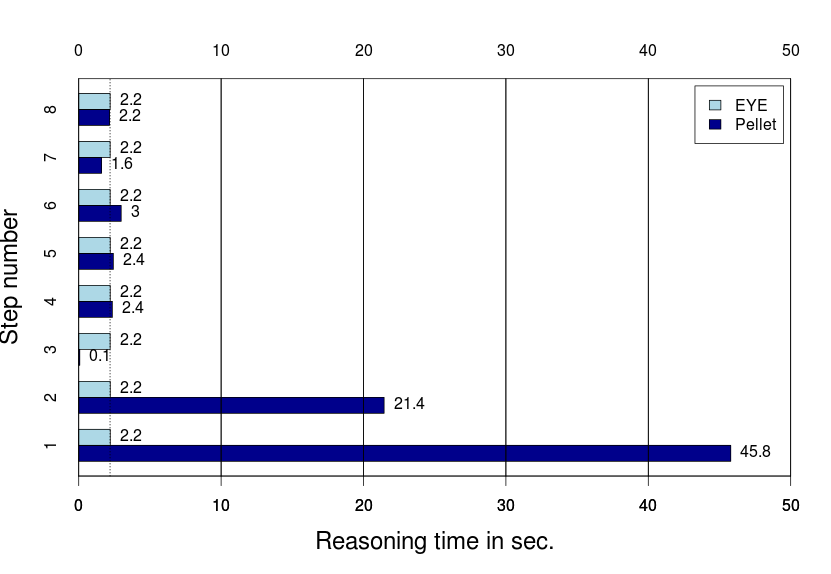
\includegraphics[width=\textwidth]{Rplot14.png}
%                 \caption{1 ward}
%                \label{fig:results1ward}
%         \end{subfigure}
%         \caption{Comparison of reasoning times (all numbers in seconds). EYE is generally faster, and more predictable.} \label{figure:results}
% \end{figure} 
  
  
\subsection{Importance and Impact}

By using rule based reasoning instead of description logic based reasoning, we create a more performant system that is more easily configurable.
The evaluation shows that the current version does not meet the performance requirements to be applied for larger datasets, however, it can already meet the constraints in a small-scaled setting, it is on average faster than more traditional approaches such as Pellet+SPARQL, and it has more robust and predictable reasoning times.

The analysis of converting a decision tree into rules shows how a rule based reasoning method is more suited to implement decision trees, and how it is as such easier configurable to make changes to the implemented decision trees.
The described analysis, being generic, can be used as a guideline for converting decision trees into rules for other use cases as well.

The results of this research are being supervised by Televic Healthcare, the leading eHealth electronics company in Belgium.
This way, the chances that the findings of this research will be commercialized are quite high, and as such, potentially improve the workload of the nurses in a hospital significantly, as elaborated on in~\ref{usecase}.

Further research will involve improving the automatic selection of relevant OWL-RL concepts.
This way, reasoning over unused concepts is avoided, which, as we believe, 
will drastically improve average reasoning times, and more importantly, will make sure that the system will 
scale a lot better than it does now.



